\label{Intro.}
Water, being ``at the centre of the planetary drama of the Anthropocene'', is essential not only for earth system processes but also in supporting development and human well-being
\cite{gleeson2020a,gleeson2020b}.
As an integral part of earth system governance, successful water governance requires a deep understanding of changes in the complex relationships between humans and water
\cite{ahlstrom2021,biermann2012,steffen2020}.
Human activities stemming from our reliance on water have profoundly modified the natural water cycle, resulting in rivers that are dominated by a hybrid of social and natural drivers
\cite{sivapalan2012,qin2014,abbott2019}.
Facing transitions from natural to human-dominated regimes, many big river basins worldwide (which are hot spots of civilization and economic growth) are urgently in need of more effective water governance
\cite{best2019,dibaldassarre2019}.

Water governance refers to the political, social, economic, and administrative systems that influence the use and management of water \cite{oecd2018, wang2017}.
For populated large river basins, missing governance means missing sustainability.
A first critical step in understanding the successes and failures of water governance is to identify the different regimes that underpin it \cite{kjellen2015, grafton2013}.
Regimes of water governance arise within linked human-water systems (based on management, institutions, and exploitation) to create local equilibria in social-ecological structures and functions
\cite{falkenmark2021,bressers2013,loch2020}.
Therefore, regime shifts sometimes lead to new water governance challenges; they are both causes and consequences of substantive changes in human-water systems.

The lack of a comprehensive but straightforward approach to identifying changes in water governance regimes represents a challenge for efforts to enhance the sustainability of water resource use.
Filling this gap, which is the aim of this paper, is important for the appropriate alignment of human and water systems (Figure~\ref{fig:framework}).
Water governance is essentially about ``who gets water, when and how''\cite{lasswell2018}. The United Nations Development Programme (UNDP) has thus suggested that three key dimensions of water use are decided by water governance directly: ``When and what water to use?'' (stress), ``How does water provide different services for human well-being?'' (purpose), and ``Who can use water equally and efficiently?'' (allocation)
\cite{undpwatergovernancefacility2016}.
First, water stress depends not only on climate (with increasing scarcity and uncertainty in many regions) but also on the increasingly insatiable demands from economic activities such as irrigation and industry; water storage can resolve some but not all of these issues
\cite{qin2019,wada2014,huang2021}.
Second, the purpose of how water services human well-being is to consider trade-offs between consumptive uses (e.g., drinking and food production) and non-consumptive uses (e.g., energy production)
\cite{liu2017,florke2018,jaeger2019}.
Third, the allocation of water across the whole basin is not only decided by regionally socio-economic and environmental context but also influenced by systematic regulation
\cite{schmandt2021,speed2013}.
Although regime shifts in water governance are related to substantive changes in any of the three dimensions, considering them separately can lead to systematic failure.

The Yellow River Basin (YRB), which contains the fifth-largest river in the world, needs integrated water governance because of geological and human history
\cite{mostern2021}.
Since the 1960s, conservation measures and the construction of regulation reservoirs and levees have contained the issues troubled by thousands of years of high sediment loads
\cite{wang2016e,song2020a}.
Decreased streamflows and water over-use in more recent times led to depletions of the over-burdened river, creating new challenges and new governance practices, including water use regulation and water transfer across basins
\cite{wang2019c}.
Today, it is still impossible to completely solve water stress, trade-offs between ecosystem services, or lopsided development in different regions in the YRB to the satisfaction of all actors; the question of ``who gets water, when and how?'' remains open for sustainable development
\cite{wohlfart2016a}.
Governance challenges induced by environmental, economic, social, and political factors have resulted in YRB being among the most intensively-governed large river basins worldwide \cite{nickum2021}.
Identifying regime shifts in water governance within the YRB can thus provide crucial insights into rapidly-changing big river basins and how governance may respond to meeting challenges to their sustainability.

% 这里我们整合了三个方向,提出了描绘流域人水关系的指数
Here, we use the three core dimensions (stress, purpose and allocation) and corresponding indicators of water governance to develop an Integrated Water Governance Index (IWGI) that can detect and describe changes in water governance at a basin-scale (see Figure~\ref{fig:framework} and methods).
% 使用案例研究
Then, by applying the index to a typical rapid-changing big river basin (the YRB), we show how to analyze the complicated water governance regimes in a comprehensive but straightforward way.
Following synthetic analyses of the changes in water demand, supply, economic outcomes, and institutions, we interpret the leading causes of the regime shifts.
% 最后总结出一般性框架
Finally, we propose a general regime transition schema that offers practical guideline for a coordinated approach to exploring the challenges faced by big river basin governance.

\begin{figure*}[!ht]
	\centering
	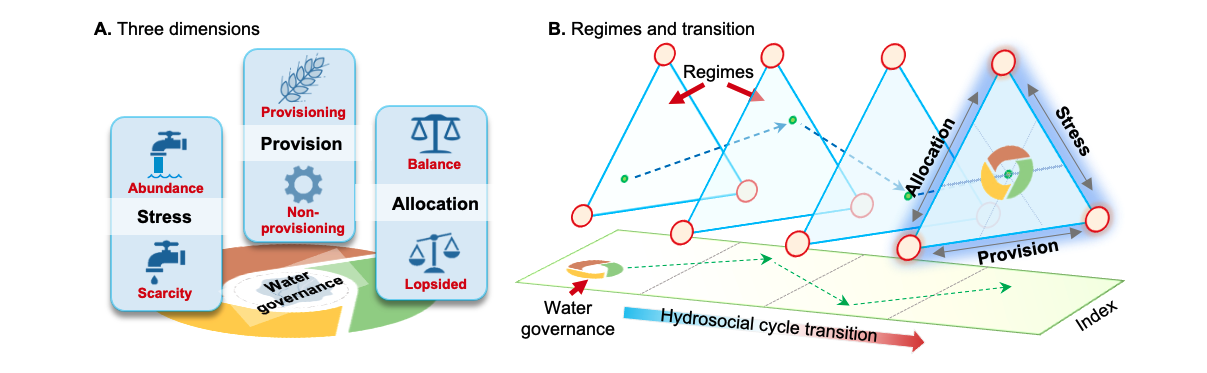
\includegraphics[width=0.9\textwidth]{main/framework.png}
	\caption{
		Identifying the water governance regimes in transitions of a hydrosocial cycle.
		\textbf{A.} Water governance has three key dimensions (stress, purpose and allocation), each of which has two potential directions (denoted in red) when changing. (1) ``stress'' of water shifts between scarcity and abundance; (2) weighting ``purpose'' of water between consumptive services or non-consumptive uses; (3) ``allocation'' changes between balanced or lopsided.
		\textbf{B.} Along with a transition in hydrosocial water cycle, water governance shifts in line with the three dimensions. Combining corresponding indicators, an abrupt change of the IWGI thus indicates a regime shift in water governance.
		% \cite{steffenTrajectoriesEarthSystem2018,abbottwatercycleAnthropocene2019,leviaHomogenizationterrestrialwater2020}.
	}
	\label{fig:framework}
\end{figure*}
